\documentclass[extendedabs]{vcom}

% VCOM - CHANGES
\usepackage[utf8]{inputenc}
\renewcommand{\abstractname}{Resumo}
\renewcommand{\refname}{Referências}

%% Enter your paper number here for the review copy
%\vcomreviewcopy{??}

\title{Visão por Computador - Reconhecimento de Objetos}

% Enter the paper's authors in order
% \addauthor{Name}{email/homepage}{INSTITUTION_CODE}
\addauthor{Leonel Peixoto - 201204919}{ei12178@fe.up.pt}{1}
\addauthor{Rodolfo Rodrigues - 200200428}{ ei12151@fe.up.pt}{2}

% Enter the institutions
% \addinstitution{Name\\Address}
\addinstitution{
 Faculdade de Engenharia\\
 Universidade do Porto\\
 Porto, Portugal
}

\runninghead{Student, Prof, Collaborator}{RECPAD Author Guidelines}

% Any macro definitions you would like to include
% These are not defined in the style file, because they don't begin
% with \bmva, so they might conflict with the user's own macros.
% The \bmvaOneDot macro adds a full stop unless there is one in the
% text already.
\def\eg{\emph{e.g}\bmvaOneDot}
\def\Eg{\emph{E.g}\bmvaOneDot}
\def\etal{\emph{et al}\bmvaOneDot}

%------------------------------------------------------------------------- 
% Document starts here
\begin{document}

\maketitle

\begin{abstract}
Trabalhos recente na área da Visão por computador permitiram o desenvolvimento de novos métodos como redes neuronais pondo os métodos clássicos em segundo plano como as Support Vector Machines (SVN). 

O objetivo principal deste projeto consiste em desenvolver um sistema que pode reconhecer e classificar um objeto presente numa imagem como sendo um objeto que pertence a uma de 10 classes diferentes. Para tal, usou-se e comparou-se dois métodos diferentes para reconhecer os objetos nas imagens. Utilizou-se uma rede neuronal convolucional e SVN usando Bag of Words (BoF) constituídos por descritores obtidos através do algoritmo SIFT. 

Os dados processados foram obtidos do dataset do CIFAR-10 do Kaggle. Chegou-se a um resultado de 78.7\% para a rede neural e 24.5\% para a melhor variante do método SVM.
\end{abstract}

%------------------------------------------------------------------------- 
\section{Introdução}
\label{sec:intro}
Um dos principais propósitos da Visão por Computador é permitir que uma máquina seja capaz de compreender e obter informação útil de imagens e vídeo, estabelecendo algoritmos para o reconhecimento e classificação de objetos, pessoas, etc. A utilização de abordagens baseadas em deep learning é a mais recente tendência e por isso é interessante realizar um comparativo com a abordagem mais tradicional de Support Vector Machines (SVM). 

O presente trabalho realiza um estudo comparativo entre uma Convolution Neural Network (CNN) e um classificador SVM associado a um extrator de features utilizando o algoritmo SIFT e um clustering em Bag of Visual Words (BoW), são avaliadas três variantes do classificador SVM: Multiclass Ranking SVM, One Against All SVM (OAA) e OAA SVM Balanced. 

O dataset utilizando neste trabalho pertence à competição CIFAR-10 do Kaggle e é composto por 60.000 imagens (50.000 imagens de treino e 10.000 imagens de teste) distribuídas por 10 categorias com 6000 imagens por categoria.

%------------------------------------------------------------------------- 
\section{Sistema Desenvolvido}
Neste trabalho foram desenvolvidas duas abordagens distintas para o sistema de reconhecimento de objetos:

%------------------------------------------------------------------------
\subsection{Rede Neuronal Convoluncional}
O sistema de reconhecimento de objetos usando deep learning foi realizado com a construção de uma rede neuronal convolucional usando as bibliotecas Keras e Theano com Python.

A rede neuronal foi sujeita a uma fase de treino com o dataset de treino do CIFAR-10 para otimizar os pesos de ligação entre cada perceptron e uma fase de avaliação com o dataset de teste do CIFAR-10.

%------------------------------------------------------------------------
\subsubsection{Arquitetura da rede}
A rede neuronal é construída por várias camadas sucessivas. As quatro primeiras camadas são do tipo convolucionais seguida por duas camadas completamente conectadas. As camadas completamente conectadas também estão completamente conectadas as camadas anteriores. Desta forma, o conjunto permite minimizar a regressão logística da função objetivo. A saída de cada camada é aplicada uma função ReLU (rectified linear unit) para aumentar a velocidade de aprendizagem. Demais, as funções ReLU permitem uma aprendizagem mesmo quando os valores de entrada não foram redimensionados.

É importante salientar que a rede de aprendizagem não requer a extração de características (features) específicas. Em vez disso, pode-se estabelecer a analogia entre as camadas iniciais convolucionais da rede e o processo de extração e representação de características. O fato de este processo ser automatizado e otimizado como parte do modelo global é um ponto muito atraente para a abordagem de deep learning.

As imagens possuem um tamanho de 32 por 32 pixéis com 3 canais de cor. A primeira e segunda camada filtram as imagens com 32 kernels de tamanho 3x3 x 2. A quarta e quinta camada são constituídas por 64 kernels 3x3. A saída da segunda e quinta camada são normalizadas com uma função de agrupamento de máximos (max pooling).

%------------------------------------------------------------------------
\subsubsection{Prevenção de \textit{overfitting}}
A rede neuronal criada é bastante grande, pois, o número total de parâmetros em todas as camadas é de vários milhões. Para o conjunto de treinamento de entrada dado, a rede foi treinada com 50 iterações. Há, portanto, um alto risco de overfitting. Para prevenir tal acontecimento, o algoritmo de treinamento emprega técnicas de "dropout", isto é, durante os passos de propagação de erro e atualização de peso, existe uma probabilidade de 0,5 que a saída de um neurônio em uma camada escondida seja definida como 0 (assim, efetivamente, impede-se de contribuir para aprendizagem nesse passo). Isso pode ser visto como treinamento de múltiplos métodos em paralelo (semelhante à validação cruzada para cada camada, onde um subconjunto dos dados é considerado de cada vez, para emular múltiplos conjuntos de dados com propriedades semelhantes, que de outra forma seriam excessivamente onerosos).

%------------------------------------------------------------------------
\subsection{Support Vector Machines}
O sistema de reconhecimento de objetos através da abordagem SVM é composto por três módulos: Extração de Features, Representação de Imagem, e Classificação. A deteção e a cálculo de descritores das features da imagem foi realizada utilizando o algoritmo SIFT. 

A representação da imagem realizou-se através de “visual words” obtidas através do clustering (k-means) das features obtidas no passo anterior, posteriormente as imagens são representadas através de histogramas dessas “visual words”. Finalmente, os histogramas são utilizados para o treino do classificador SVM. Os três módulos foram desenvolvidos utilizando a versão 2.4 da biblioteca OpenCV.

%------------------------------------------------------------------------
\subsubsection{Extração de Features}
O módulo de extração de features das imagens de teste é realizado utilizando o algoritmo SIFT para a deteção das features e cálculo dos descritores das features. O produto deste módulo é um conjunto de vetores normalizados que serve de base à definição do vocabulário de “visual words”.

%------------------------------------------------------------------------
\subsubsection{Representação de Imagem}
O módulo anterior gera descritores das features das imagens do dataset que serão utilizados no processo de clustering do presente módulo, através do algoritmo k-means, os descritores são agrupados em clusters que representam uma “visual word” e conjunto dos clusters é o vocabulário do nosso modelo de Bag of Words.

A definição do vocabulário do nosso modelo de Bag of Words permite a representação das imagens de treino do dataset através de um histograma das “visual words”, permitindo a aplicação da metodologia SVM a este espaço de features de dimensão igual à dimensão do vocabulário do modelo BoW.

Uma das principais variáveis desta abordagem é a dimensão do vocabulário (número de clusters) a usar, de forma a encontrar uma dimensão que produzisse resultados aceitáveis foram testados vários valores. 

%------------------------------------------------------------------------
\subsubsection{Classificação}
A representação em histograma das imagens do dataset foram utilizadas no treino do classificador SVM, dado que neste trabalho de reconhecimento de objetos existem 10 classificações distintas foram elaboradas três variantes do classificador SVM: Multiclass ranking SVM, One Against All SVM (OAA) e OAA SVM Balanced. 

A variante Multiclass Ranking SVM utiliza a função de decisão para tentar classificar todas as 10 classes existentes, a OAA SVM possui um classificador binário SVM para cada classe para separar os membros dessa classe de todas as outras classes. Por fim, como no dataset de 60.000 imagens existem 6.000 imagens por classe, um subset de treino terá em média apenas 10 \% de imagens de cada classe, o que no caso da variante OAA SVM se traduz num set de treino desequilibrado para cada um dos classificadores binários. Assim, elaborou-se uma terceira variante OAA SVM Balanced onde se garante que 50 \% do subset de treino são imagens da classe que o classificador binário pretende identificar.

Na variante Multiclass Ranking SVM, o classificador SVM atribui directamente uma classe às imagens que processa, mas no caso das variantes OAA SVM e OAA SVM Balanced esta classificação não é direta porque é necessário conjugar os resultados dos vários classificadores binários, bem como, resolver situações em que vários classificadores aceitam ou todos rejeitam uma determinada imagem. Nestas duas variantes, a classificação atribuída à imagem coincide com a classe do classificador binário com o maior valor da função de decisão (maior distância à fronteira do classificador SVM).

%------------------------------------------------------------------------
\section{Resultados}

%------------------------------------------------------------------------
\subsection{Rede Neuronal Convoluncional}

\begin{figure}[h]
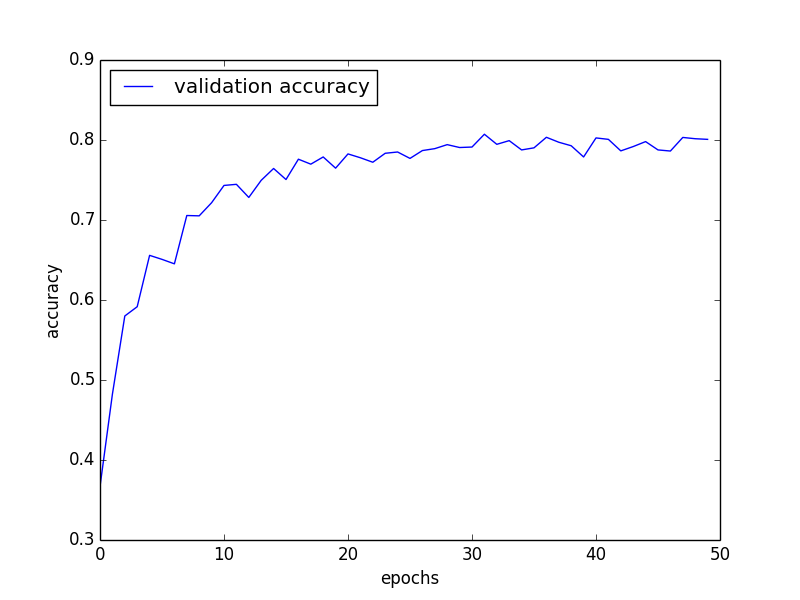
\includegraphics[width=\linewidth]{images/obj_rec_graph_50.png}
\caption{Variação da precisão da CNN ao longo dos ciclos de treino}
\label{fig:graph2}
\end{figure}

O treino da rede neuronal convoluncional permitiu obter uma precisão de 78.7\%, um valor substancialmente superior ao obtido na abordagem SVM. Foram testadas algumas configurações alternativas da rede neuronal, mas este processo não foi exaustivo porque o processo de treino da rede é extremamente demorado, especialmente quando não é possível utilizador o processador GPU. Por outro lado, o processo de classificação das imagens é bastante rápido. O tempo necessário para o treino da rede é a sua principal desvantagem, sendo mesmo mais longo do que o já demorado SVM.

%------------------------------------------------------------------------
\subsection{Support Vector Machines}

\begin{figure}[h]
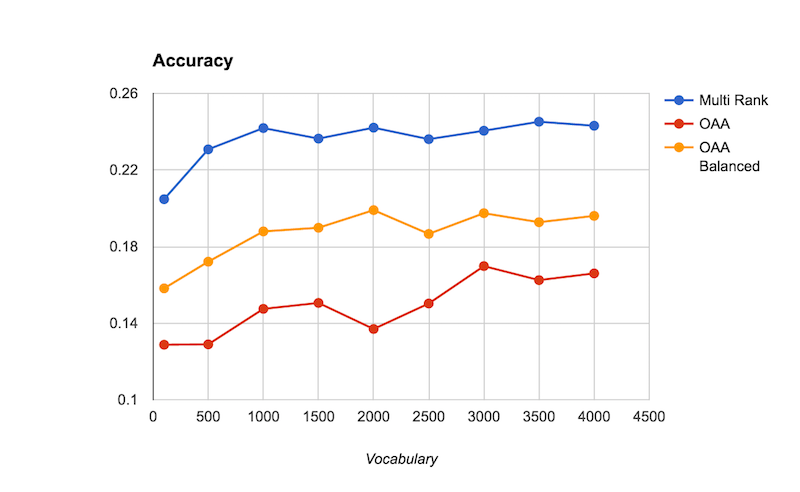
\includegraphics[width=\linewidth]{images/svn_graph.png}
\caption{Variação da precisão das abordagens SVM para diferentes dimensões de vocabulário}
\label{fig:graph1}
\end{figure}

A variante Multiclass ranking SVM permitiu obter o valor mais elevado de precisão 24.5\% com um vocabulário de 3500 palavras. 

Na variante One Against All SVM obteve-se 16.9\% com um vocabulário de 3000 palavras e com um dataset de treino equilibrado consegue-se uma melhoria de precisão para 19.9\% com um vocabulário de 2000 palavras. 

A variante Multiclass ranking SVM apesar de só possuir um classificador SVM tem um processo de treino mais lento do que as outras variantes constituídas por dez classificadores binários SVM.

%------------------------------------------------------------------------
\section{Conclusões}
A rede neuronal convoluncional teve uma prestação superior às variantes da abordagem SVM, o que está de acordo com o que era esperado apesar de a diferença entre as prestações ser superior às nossas expectativas. O SVM tem dificuldade em processar datasets com um elevado número de dimensões porque a maior parte desses espaços de features são constituídos por dados que não são separáveis. Como o fundamento do modelo SVM é a procura de um hiperplano que separe os dados desse espaço de features, se os dados não são separáveis é geometricamente impossível encontrar uma solução. 

A rede neuronal convoluncional não tem estas limitações apesar de que o treino de uma rede é uma tarefa bastante dispendiosa ao nível do tempo e dos recursos. É importante referir que é difícil antever os resultados de uma determinada rede neuronal com base na sua estrutura e nas características das suas camadas.

Concluímos que, nos problemas de reconhecimento de objetos, as redes neuronais convoluncionais têm uma clara vantagem sobre as abordagens mais clássicas mesmo considerando o maior custo do seu processo de treino.

%------------------------------------------------------------------------
\section{Melhoramentos Futuros}
Relativamente às variantes da abordagem SVM seria interessante realizar o processo de treino dos classificadores SVM de forma a obter os parâmetros ótimos com base na estimativa de cross-validation. Outra melhoria do trabalho realizado seria a utilização de um dataset maior na variante OAA SVM Balance porque o dataset utilizado para cada um dos classificadores SVM desta variante é um quinto do dataset utilizado nas outras duas variantes. 

No caso da rede neuronal convoluncional, como já foi referido, devido à dificuldade em prever o impacto da estrutura e da configuração da rede nos resultados seria importante despender mais algum tempo na sua otimização.  

%------------------------------------------------------------------------
\bibliography{egbib}{}
\bibliographystyle{plain}

\end{document}
